\documentclass[11pt, a4paper]{article}

\usepackage[english]{babel}
\usepackage{sleek}
\usepackage{common}

\title{Introduction to Artificial Intelligence (INFO8006)}
\subtitle{Exercise session 6}

\def\ReLU{\mathrm{ReLU}}

\begin{document}

\maketitle

\begin{thbox}{Multilayer perceptron}
    For an \thighlight{input vector} $\mathbf{x} \in \mathbb{R}^d$ and  \thighlight{activation function} $\sigma(.)$, a MLP with $L$ layers can be written as 
    \begin{align*}
        \mathbf{h}_0 &= \mathbf{x}\\
        \mathbf{h}_1 &= \sigma(\mathbf{W}_1^T\mathbf{h}_0 + \mathbf{b}_1)\\
        &\vdots\\
        \mathbf{h}_L &= \sigma(\mathbf{W}_L^T\mathbf{h}_{L-1} + \mathbf{b}_L)\\
        \mathbf{y} &= \mathbf{h}_L
    \end{align*}
    with $\mathbf{h}_l \in \mathbb{R}^{q_l}$ defined as the the \thighlight{hidden vector}, $\mathbf{W}_l \in \mathbb{R}^{q_{l-1} \times q_l}$ the \thighlight{weight matrix} and $\mathbf{b}_l \in \mathbb{R}^{q_l}$ the \thighlight{bias vector} of the $l$-th layer.
\end{thbox}
\begin{thbox}{Training loop}
    For a given \thighlight{input-output training pair} $(x, y)$, a \thighlight{neural network} $\Phi_\theta(.)$ \thighlight{parameterized} by $\theta$, a \thighlight{loss function} $\mathcal{L}(.)$ and a \thighlight{learning rate} $\lambda$:
    \begin{enumerate}
        \item Compute all intermediate values in the network for the given input $x$ up to the output prediction $\hat{y} = \Phi_\theta(x)$. This is known as the \thighlight{forward pass}.
        \item Compute the symbolic \thighlight{gradient} of the loss w.r.t. every parameters $g_i(.) = \frac{\partial \mathcal{L}}{\partial \theta_i}$ using the chain rule.
        \item Evaluate the loss for your training point as $\mathcal{L}(y,\hat{y})$.
        \item Backpropagate the loss and the activations through the network to compute the gradient values $g_i$. This is known as the \thighlight{backward pass}.
        \item Update every parameter using their gradient as 
        $$
        \theta_i \leftarrow \theta_i - \lambda g_i.
        $$
    \end{enumerate}
\end{thbox}
\begin{thbox}{Universal approximation theorem}
    The \thighlight{universal approximation theorem} states that a single-hidden-layer network with a finite number of hidden units can approximate any continuous function on a compact subset of $\mathbb{R}^d$ to arbitrary accuracy.
\end{thbox}
\textbf{In session exercices}: Ex. 1, Ex. 2
\newpage

\section{Escape game (January 2022)}

A new virtual escape game came out, and you decide to play it. You arrive in a $5 \times 5$ grid world where each cell $(x, y)$ is a room with doors leading to the adjacent rooms. The game's goal is to reach the exit room as fast as possible, but its position is unknown. Furthermore, some regions of the world are full of riddles, and crossing rooms in these regions takes longer. Fortunately, a leaderboard with the players' best times is provided, starting from a few different rooms. Due to rounding errors, you assume that the best times reported in the leaderboard are measurements affected by additive Gaussian noise $\N(0, 1)$.

\begin{table}[h]
    \centering
    \begin{tabular}{c|cc}
        \toprule
        $i$ & Starting room & Measured best time \\
        \midrule
        1 & $(4, 5)$ & $2.0$ \\
        2 & $(5, 3)$ & $3.5$ \\
        3 & $(3, 3)$ & $4.5$ \\
        4 & $(4, 1)$ & $7.0$ \\
        5 & $(1, 2)$ & $8.5$ \\
        \bottomrule
    \end{tabular}
\end{table}

From the leaderboard, you wish to learn a heuristic approximating the best time to get to the exit, starting from room $(x, y)$. You decide to use a small neural network as approximator, described by the following parametric function,
\begin{align*}
    h(x, y; \phi) & = \text{ReLU}(x w_1 + y w_2 + w_3) + \text{ReLU}(x w_4 + y w_5 + w_6) \\
    \text{ReLU}(x) & = \max(x, 0) ,
\end{align*}
where $\phi = (w_1, w_2, w_3, w_4, w_5, w_6)$ is the set of parameters/weights of the neural network.

\begin{enumerate}
    \item Among the following sets of parameters ($A$, $B$ or $C$), which one would you use? Justify your answer.

    \begin{table}[h]
        \centering
        \begin{tabular}{c|cccccc}
            \toprule
            Set & $w_1$ & $w_2$ & $w_3$ & $w_4$ & $w_5$ & $w_6$ \\
            \midrule
            $\phi_A$ &$-1.5$ & $1$ & $4$ & $1$ & $-1.5$ & $6$ \\
            $\phi_B$ &$-1$ & $1.5$ & $3$ & $0$ & $-1$ & $4$ \\
            $\phi_C$ &$-2$ & $0.5$ & $4.5$ & $1.5$ & $0$ & $5$ \\
            \bottomrule
        \end{tabular}
    \end{table}

    \begin{solution}
        A set of parameters is better than another if it explains the data better, that is if the likelihood is higher. Our task is to find the set of parameters that maximizes the likelihood under the assumed probability model. In our case, the data $d$ is the leaderboard and consists of independent position-time tuples $(x_i, y_i, t_i)$. From the statement, we gather that the (best) time $t$ is a function of the starting position $(x, y)$, approximated by a neural network $h(x, y; \phi)$. We also learn that our time measurements are affected by Gaussian noise.
        \begin{align*}
            \phi_{\text{MLE}} & = \arg\max_\phi p(d | \phi) \\
            & = \arg\max_\phi \prod_{i=1}^5 p(x_i, y_i, t_i | \phi) \\ \displaybreak
            & = \arg\max_\phi \prod_{i=1}^5 p(t_i | x_i, y_i, \phi) \, p(x_i, y_i) \\
            & = \arg\max_\phi \prod_{i=1}^5 \N(t; h(x, y; \phi), 1) \\
            & = \arg\max_\phi \sum_{i=1}^5 \log \sbk*{\frac{1}{\sqrt{2 \pi}} \exp \rbk*{-\frac{(t_i - h(x_i, y_i; \phi))^2}{2}}} \\
            & = \arg\min_\phi \sum_{i=1}^5 (t_i - h(x_i, y_i; \phi))^2
        \end{align*}
        Now that we have an objective $L(\phi)$ to minimize, we can evaluate it for each of the proposed sets and select the best one.
        \begin{align*}
            L(\phi_A) & = \sum_{i=1}^5 (t_i - h(x_i, y_i; \phi_A))^2 = (2.0 - 5.5)^2 + (3.5 - 6.5)^2 + \dots = 29.75 \\
            L(\phi_B) & = 35.75 \\
            L(\phi_C) & = 205.25
        \end{align*}
        The best set is $\phi_A$.
    \end{solution}

    \item You now assume a Gaussian prior $\N(0, 1)$ on each parameter. Which set of parameters in the table above would you now choose? Justify your answer.

    \begin{solution}
        Now that we hold a prior belief on the parameters, our task is to find the most likely set of parameters given the data, that is maximum a posteriori (MAP) estimation.
        \begin{align*}
            \phi_{\text{MAP}} & = \arg\max_\phi p(\phi | d) \\
            & = \arg\max_\phi p(d | \phi) p(\phi) \\
            & = \arg\max_\phi \prod_{i=1}^5 p(x_i, y_i, t_i | \phi) \prod_{j=1}^6 p(w_j) \\
            & = \arg\max_\phi \prod_{i=1}^5 \N(t; h(x, y; \phi), 1) \prod_{j=1}^6 \N(w_j; 0, 1) \\
            & = \arg\min_\phi \sum_{i=1}^5 (t_i - h(x_i, y_i; \phi))^2 + \underbrace{\sum_{j=1}^6 (w_j)^2}_{\norm{\phi}^2}
        \end{align*}
        Here again, we have an objective $L'(\phi)$ to minimize, which we evaluate for each of the proposed sets.
        \begin{align*}
            L'(\phi_A) & = L(\phi_A) + \sum_{j=1}^6 (w_j)^2 = 29.75 + (-1.5)^2 + (1)^2 + \dots = 88.25 \\
            L'(\phi_B) & = 65.0 \\
            L'(\phi_C) & = 257.0
        \end{align*}
        The best set is $\phi_B$.
    \end{solution}

    \item Discuss the procedure you would implement on a computer to find the optimal set of parameters, had the table above not been provided.

    \begin{solution}
        If the table is not provided, it is intractable to evaluate and compare all possible sets of parameters. However, we still want to minimize the MLE (or MAP) objective $L(\phi)$. We can improve a set of parameters $\phi$ by following the opposite of the objective's gradient $\nabla_{\! \phi} L(\phi)$, \ie{} performing \emph{gradient descent} steps
        \begin{equation*}
            \phi \gets \phi - \gamma \nabla_{\! \phi} L(\phi) ,
        \end{equation*}
        where $\gamma$ is the learning rate.
    \end{solution}
\end{enumerate}

\newpage

\section{Neural network representations (CS188, Spring 2024)}
You are given a number of functions (a-h) of a single variable, $x$, which are graphed below. For each network structure proposed afterwards, indicate which functions they are able to represent. When possible, indicate appropriate values for the parameters.

\begin{figure}[h]
    \centering
    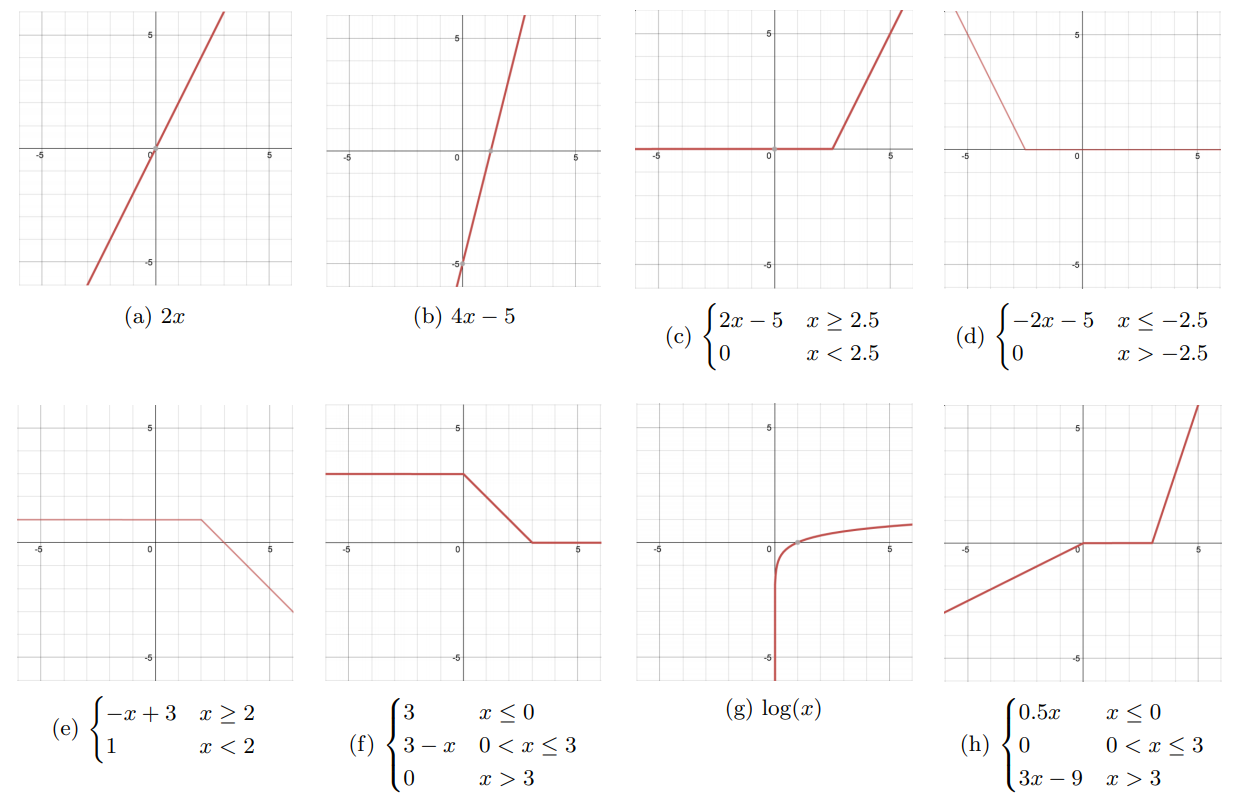
\includegraphics[width=.9\linewidth]{figures/nnfunctions.png}
\end{figure}

\begin{enumerate}
    \item We start with a linear transformation of the scalar input $x$, weight
$w$, and output $y$, such that $y = wx$.
    \begin{figure}[h!]
    \centering
    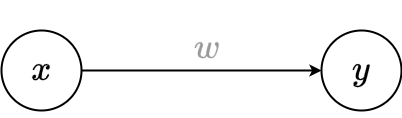
\includegraphics[width=.4\linewidth]{figures/linearnet.png}
\end{figure}

    \begin{solution}
        This network can only represent (a), with $w = 2$. Since there is no bias term, the line must pass through the origin.
    \end{solution}
    
    \item We then introduce a bias term $b$, such that $y = wx+b$.
    \begin{figure}[h!]
    \centering
    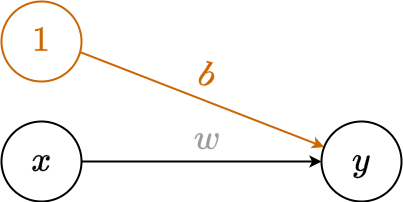
\includegraphics[width=.4\linewidth]{figures/affinenet.png}
\end{figure}

    \begin{solution}
        (a) with $w = 2$ and $b = 0$, and (b) with $w = 4$ and $b = -5$.
    \end{solution}
    
    \item We now introduce a non-linearity $\sigma (.)$ into the network. We use the ReLU non-linearity, which has the form ReLU(x) = max(0, x).
    \begin{figure}[h!]
    \centering
    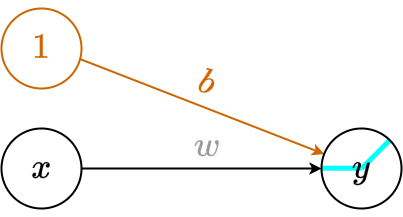
\includegraphics[width=.4\linewidth]{figures/onerelu.png}
\end{figure}

    \begin{solution}
        With the output coming directly from the ReLU, this cannot produce any values less than zero. It can produce (c) with $w = 2$ and $b = -5$, and (d) with $w = -2$ and $b = -5$.
    \end{solution}
    
    \item Now we consider neural networks with multiple affine transformations, as depicted below. 
    \begin{figure}[h!]
    \centering
    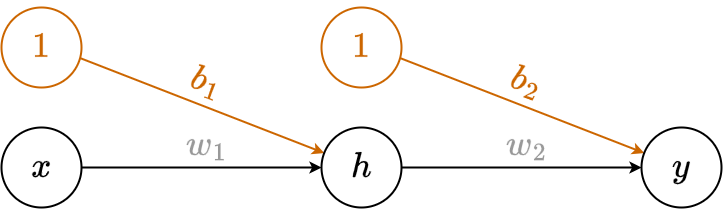
\includegraphics[width=.6\linewidth]{figures/doubleaffine.png}
\end{figure}

    \begin{solution}
        Applying multiple affine transformations (with no non-linearity in between) is not any more powerful than a single affine function: $w_2(w_1x + b_1) + b_2 = w_2w_1x + w_2b_1 + b_2$, so this is just a affine function with different coefficients. The functions we can represent are the same as in 1, if we choose $w_1 = w$, $w_2 = 1$, $b_1 = 0$, $b_2 = b$: (a) with $w_1 = 2$, $w_2 = 1$, $b_1 = 0$, $b_2 = 0$, and (b) with $w_1 = 4$, $w_2 = 1$, $b_1 = 0$, $b_2 = -5$.
    \end{solution}
    
    \item We now add a ReLU non-linearity to the network between the affine transformations.
    \begin{figure}[h!]
    \centering
    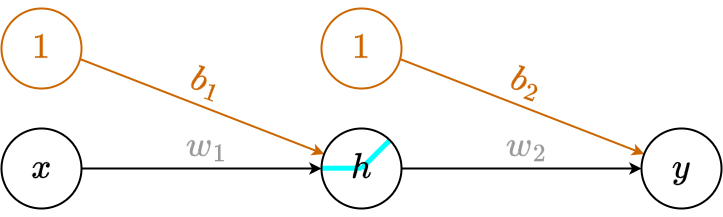
\includegraphics[width=.6\linewidth]{figures/onehidden.png}
\end{figure}

    \begin{solution}
        (c), (d), and (e). The affine transformation after the ReLU is capable of stretching (or flipping) and shifting the ReLU output in the vertical dimension. The parameters to produce these are: (c) with $w_1 = 2$, $b_1 = -5$, $w_2 = 1$, $b_2 = 0$, (d) with $w_1 = -2$, $b_1 = -5$, $w_2 = 1$, $b_2 = 0$, and (e) with $w_1 = 1$, $b_1 = -2$, $w_2 = -1$, $b_2 = 1$.
    \end{solution}
    
    \item Now we add another hidden layer to the network, as depicted below. You do not have to guess parameters values anymore.
    \begin{figure}[h!]
    \centering
    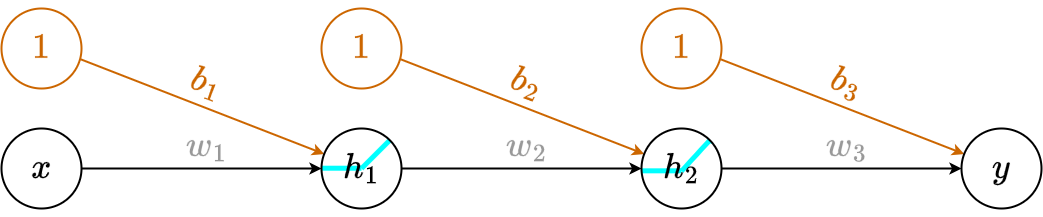
\includegraphics[width=.8\linewidth]{figures/twolhidden.png}
\end{figure}

    \begin{solution}
        (c), (d), (e), and (f). The network can represent all the same functions as Q5 (because note that we could have $w_2 = 1$ and $b_2 = 0$). In addition it can represent (f): the first ReLU can produce the first flat segment, the affine transformation can flip and shift the resulting curve, and then the second ReLU can produce the second flat segment (with the final affine layer not doing anything). Note that (h) cannot be produced since its line has only one flat segment (and the affine layers can only scale, shift, and flip the graph in the vertical dimension; they can’t rotate the graph).
    \end{solution}
    
    \item We’d like to consider using a neural net with just one hidden layer, but larger. Let’s first consider using just two affine functions, with no nonlinearity in between. You do not have to guess parameters values anymore.
    \begin{figure}[h!]
    \centering
    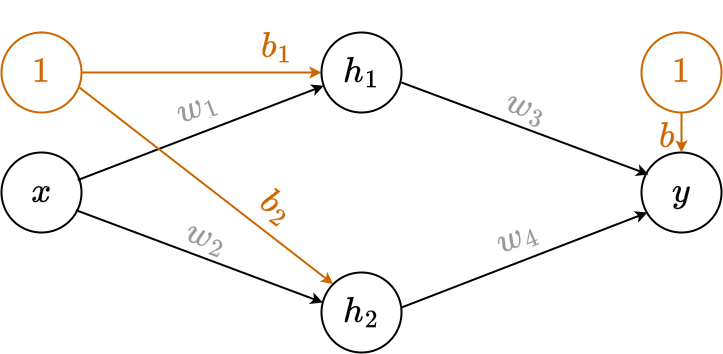
\includegraphics[width=.7\linewidth]{figures/2hiddenlin.png}
\end{figure}

    \begin{solution}
        (a) and (b). With no non-linearity, this reduces to a single affine function (in the same way as Q4).
    \end{solution}
    
    \item Now we’ll add a non-linearity between the two affine layers, to produce the neural network below with a
hidden layer of size 2. You do not have to guess parameters values anymore.
    \begin{figure}[h!]
    \centering
    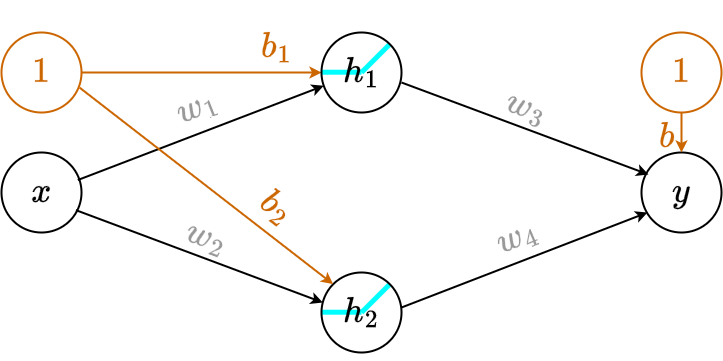
\includegraphics[width=.7\linewidth]{figures/2hiddennl.png}
\end{figure}

    \begin{solution}
        All functions except for (g). Note that we can recreate any network from (5) by setting $w_4$ to 0, so this allows us to produce (c), (d) and (e). To produce the rest of the functions, note that $h_1$ and $h_2$ will be two independent functions with a flat part lying on the x-axis, and a portion with positive slope. The final layer takes a weighted sum of these two functions. To produce (a) and (b), the flat portion of one ReLU should start at the point where the other ends ($x = 0$ for (a), or $x = 1$ for (b). The final layer then vertically flips the ReLU sloping down and adds it to the one sloping up, producing a single sloped line. To produce (h), the ReLU sloping down should have its flat portion end (at $x = 0$ before the other’s flat portion begins (at $x = 3$). The down-sloping one is again flipped and added to the up-sloping. To produce (f), both ReLUs should have equal slope, which will cancel to produce the first flat portion above the x-axis.
    \end{solution}

    \item Are there functions that can't be represented by all proposed networks? If yes, explain why and what you would need to model them.
    
    \begin{solution}
        Yes, function (g) cannot be modeled. We first see that the function is smooth and representing it only with few ReLU activations is not enough. We should probably use smoother activations like SiLU, tanh, ... (see slide 48 of the "Machine learning and neural networks" lecture).\\
        
        However, we remember the universal approximation theorem which states that a single-hidden-layer network with a finite number of hidden units can approximate any continuous function on a compact subset of $\mathbb{R}^d$ to arbitrary accuracy. Then, adding sufficient amount of hidden units of the 1-layer network of part 8 should be sufficient.\\

        Note that the logarithm function is only defined on $\mathbb{R}^+$. If our network is made of activation functions defined on $\mathbb{R}$, we will never be able to restrict the domain of the learned function to only real positive. However, you can be as accurate as you want on the desired domain, but it makes no sense to evaluate your network elsewhere for this problem.
    \end{solution}
\end{enumerate}

\newpage 

\section{ReLU}

For each of the piecewise-linear functions below, write a function $y = f(x)$ as a composition of sums ($+, -$), ReLU ($\mathrm{ReLU}(x) = \max(x, 0)$) non-linearities, and real parameters (weights and biases) that exactly matches the function over $\R$.

\begin{center}
    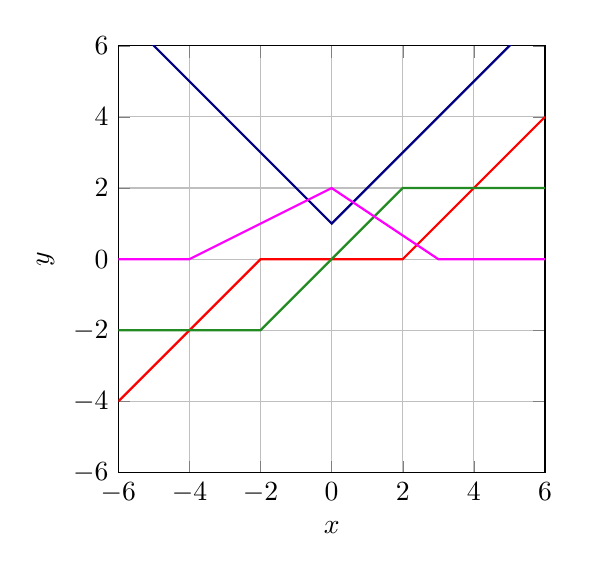
\begin{tikzpicture}[
        declare function={
            relu(\x) = max(\x, 0);
            a(\x) = relu(\x) + relu(-\x) + 1;
            b(\x) = relu(\x - 2) -relu(-\x - 2);
            c(\x) = relu(-relu(-\x + 2) + 4) - 2;
            d(\x) = relu(-relu(2 * \x / 3) - relu(-\x / 2) + 2);
        }
    ]
        \begin{axis}[
            width=7cm,
            height=7cm,
            grid=major,
            ymin=-6, ymax=6, ylabel=$y$,
            xmin=-6, xmax=6, xlabel=$x$,
            domain=-6:6,
            samples=12 + 1,
        ]
            \addplot[NavyBlue, thick] {a(x)};
            \addplot[Red, thick] {b(x)};
            \addplot[ForestGreen, thick] {c(x)};
            \addplot[Fuchsia, thick] {d(x)};
        \end{axis}
    \end{tikzpicture}
\end{center}

For example, $y = \ReLU(x + 2) - \ReLU(-2x)$ is a valid function.

\begin{solution}
    \begin{enumerate}
        \item \textcolor{NavyBlue}{$y = \ReLU(x) - \ReLU(-x) + 1$}
        \item \textcolor{Red}{$y = \ReLU(x - 2) - \ReLU(-x - 2)$}
        \item \textcolor{ForestGreen}{$y = \ReLU(-\ReLU(-x + 2) + 4) - 2$}
        \item \textcolor{Fuchsia}{$y = \ReLU(-\ReLU(\frac{2}{3} x) - \ReLU(-\frac{1}{2} x) + 2)$}
    \end{enumerate}
\end{solution}

\newpage

\section{Classification (CS188, Spring 2024)}
Consider the following simple neural network for binary classification. Here $x$ is a single real-valued input feature with an associated class $y$ (0 or 1). There are two weight parameters $w_1$ and $w_2$, and non-linearity functions $g_1$ and $g_2$. The network will output a value $a_2$ between 0 and 1, representing the probability of being in class 1. We will be using a loss function $\mathcal{L}$ to compare the prediction $a_2$ with the true class $y$.

\begin{figure}[h!]
    \centering
    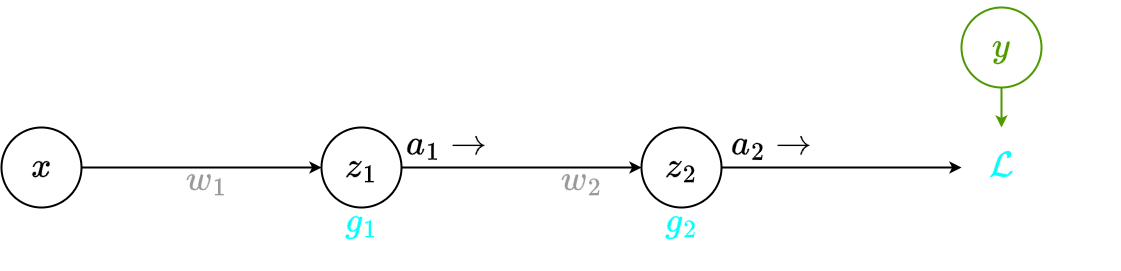
\includegraphics[width=\linewidth]{figures/classif_2.png}
\end{figure}

\begin{enumerate}
    \item Write down the forward pass on this network, writing the output values for each node $z_1$, $a_1$, $z_2$ and $a_2$ in terms of the node’s input values.
    
    \begin{solution}
        \begin{align*}
            z_1 &= w_1 x\\
            a_1 &= g_1(z_1) = g_1(w_1 x)\\
            z_2 &= w_2 a_1 = w_2 g_1(w_1 x)\\
            a_2 &= g_2(z_2) = g_2(w_2 g_1(w_1 x))
        \end{align*}
    \end{solution}
    
    \item Derive the arguments of the loss $\mathcal{L}(a_2, y)$ in terms of the input $x$, weights $w_i$, and activation functions $g_i$.

    \begin{solution}
        The argument $a_2$ has been derived in the previous question. We have 
        $$
        a_2 = g_2(w_2 g_1(w_1 x)).
        $$
        For the other input $y$, the latter is given as input of the problem. Indeed, in supervised learning, we assume access to a training dataset made of input-output pairs $\{(x_i, y_i)\}^N$ where $y_i$ acts as a target for the network.
    \end{solution}

    \item Using the chain rule, differentiate $\mathcal{L}$ w.r.t. $w_2$. Write your expression as a product of partial derivatives at each node: i.e. the partial derivative of the node’s output with respect to its inputs. (Hint: the series of expressions you wrote in part 1 will be helpful; you may use any of those variables.)

    \begin{solution}
        $$
        \dfrac{\partial \mathcal{L}}{\partial w_2} = \dfrac{\partial \mathcal{L}}{\partial a_2} \dfrac{\partial a_2}{\partial z_2} \dfrac{\partial z_2}{\partial w_2} 
        $$
    \end{solution}

    \item Motivate a choice for the output activation function $g_2$ given the nature of the problem. Motivate also a loss function. Give the expression of the gradients of both functions w.r.t. to their inputs.

    \begin{solution}
        From the statement
        \begin{enumerate}
            \item we know that we are in a classification problem (specifically, a binary classification),
            \item we know that the output $a_2$ should be between 0 and 1 and represents the probability $p(Y = 1 \mid x)$.
        \end{enumerate}
        From (b), we have $a_2: \mathbb{R} \mapsto [0,1]$. A typical choice that fulfill this requirement is the sigmoid function $\sigma(z) = \dfrac{1}{1 + e^{-z}}$. The gradient of the sigmoid w.r.t. its input is 
        $$
        \dfrac{\partial \sigma(z)}{\partial z} = \dfrac{e^{-z}}{(1 + e^{-z})^2} = \sigma(z)\sigma(-z) = \sigma(z)(1-\sigma(z)).
        $$
        For the loss function, either we remember the cross-entropy loss seen in the theoretical lecture, or we compute it from maximum likelihood estimation.\\

        The likelihood of a pair $(x, y)$ can be derived from our model as
        $$
        \begin{cases}
            \text{if } y = 1\  \text{ then }\ P(Y = y \mid x) = \text{NN}_{\theta}(x)\\
            \text{if } y = 0\  \text{ then }\ P(Y = y \mid x) = 1 -\text{NN}_{\theta}(x)
        \end{cases}
        $$
        where $\text{NN}_{\theta}$ is the neural network parameterized by $\theta = [w_1, w_2]$. Denoting $\text{NN}_{\theta}(x) = a_2$, the likelihood expression for one pair can be reformulated as 
        $$
        L(x, y; \theta) = y\log a_2 + (1-y) \log (1 - a_2).
        $$
        Since we want to maximize the likelihood, but minimize the loss, we can set the latter to
        $$
        \mathcal{L}(a_2, y) = -y\log a_2 - (1-y) \log (1 - a_2)
        $$
        which corresponds to the binary cross-entropy loss. The gradient of the loss w.r.t. $a_2$ is
        $$
        \dfrac{\partial \mathcal{L}(a_2, y)}{\partial a_2} = -\dfrac{y}{a_2} + \dfrac{(1-y)}{(1-a_2)} = \dfrac{a_2 - y}{a_2(1- a_2)}.
        $$
    \end{solution}
    
    \item We set the loss function to the binary cross-entropy $$\mathcal{L}(a_2, y) = -y\log a_2 - (1-y) \log (1 - a_2),$$ and $g_1$ and $g_2$ are both sigmoid functions $\sigma(z) = \frac{1}{1 + e^{-z}}$. If you made this choice in the previous question, use your results to get the expression of $\frac{\partial \mathcal{L}}{\partial w_2}$. Otherwise, start by expressing $\frac{\partial \sigma(z)}{\partial z}$ and $\frac{\partial \mathcal{L}}{\partial a_2}$.

    \begin{solution}
        We first miss $\frac{\partial z_2}{\partial w_2}$ which is
        $$
            \frac{\partial z_2}{\partial w_2} =  \frac{\partial}{\partial w_2} (w_2a_1) = a_1.
        $$
        Plugging all the partial derivatives to the expression found in part 3, we have
        \begin{align*}
            \dfrac{\partial \mathcal{L}}{\partial w_2} &= \dfrac{a_2 - y}{a_2 (1 - a_2)} g_2(z_2)(1 - g_2(z_2)) a_1 \\
            &= \dfrac{a_2 - y}{a_2 (1 - a_2)} a_2(1 - a_2) a_1\\
            &= (a_2 - y) a_1
        \end{align*}
    
    \end{solution}

    \item Now use the chain rule to express $\frac{\partial \mathcal{L}}{\partial w_1}$ as a product of partial derivatives at each node of interest.

    \begin{solution}
        $$
        \frac{\partial \mathcal{L}}{\partial w_1} = \dfrac{\partial \mathcal{L}}{\partial a_2} \dfrac{\partial a_2}{\partial z_2} \dfrac{\partial z_2}{\partial a_1} \dfrac{\partial a_1}{\partial z_1} \dfrac{\partial z_1}{\partial w_1}
        $$
    \end{solution}

    \item Finally, write $\dfrac{\partial \mathcal{L}}{\partial w_1}$ in terms of $x$, $y$, $w_i$, $a_i$, $z_i$.

    \begin{solution}
        We first need to compute 
        $$
            \frac{\partial a_1}{\partial z_1} =  g_1(z_1)(1 - g_1(z_1)) = a_1(1-a_1)
        $$
        similarly to $\frac{\partial a_2}{\partial z_2}$, and
        $$
            \frac{\partial z_1}{\partial w_1} =  \frac{\partial}{\partial w_1} (w_1x) = x.
        $$
        Then, we get 
        $$
            \frac{\partial \mathcal{L}}{\partial w_1} = (a_2 - y)w_2 a_1(1-a_1)x.
        $$
    \end{solution}

    \item What is the gradient descent update for $w_1$ with step-size $\lambda$ in terms of the values computed above?

    \begin{solution}
        $$
        w_1 \leftarrow w_1 - \lambda (a_2 - y)w_2 a_1(1-a_1)x.
        $$
        You see here the importance of the forward pass. Iteratively, when receiving the input $x$, we compute all the intermediate activations (here, $a_1$ and $a_2$) and the loss (given $y$). Then, we propagate backward (from the output to the input) the values following the chain rule for the gradient of the loss w.r.t. parameters of interest. Finally, we update the parameters using the computed gradient.
    \end{solution}
\end{enumerate}
\newpage

% neural networks

\section{Training loop (INFO8006, January 2024)}
Let us consider a neural network $f$ with one hidden layer taking as input a scalar $x \in \mathbb{R}$ and producing as output a scalar $y=f(x;\theta) \in \mathbb{R}$. The neural network is defined as $$f(x; \theta) = w_1 \text{ReLU}(w_2 x + w_3) + w_4 \text{ReLU}(w_5 x + w_6) + w_7 \text{ReLU}(w_8 x + w_9),$$ where $\theta = (w_1, w_2, w_3, w_4, w_5, w_6, w_7, w_8, w_9)$ is the set of parameters and $\text{ReLU}(x) = \max(x, 0)$ is the rectified linear unit function.

\begin{enumerate}
    \item Draw the computation graph representing the neural network and the flow of information from inputs to outputs. Your diagram should be a directed graph that follows the following conventions:
    \begin{itemize}
        \item circled nodes correspond to variables (input, output, parameters or intermediate variables),
        \item squared nodes correspond to primitive operations (addition, multiplication, ReLU) and produce an intermediate variable as output,
        \item directed edges correspond to the flow of information, from inputs to outputs.
    \end{itemize}

    \begin{solution}
        \begin{figure}[h!]
            \centering
            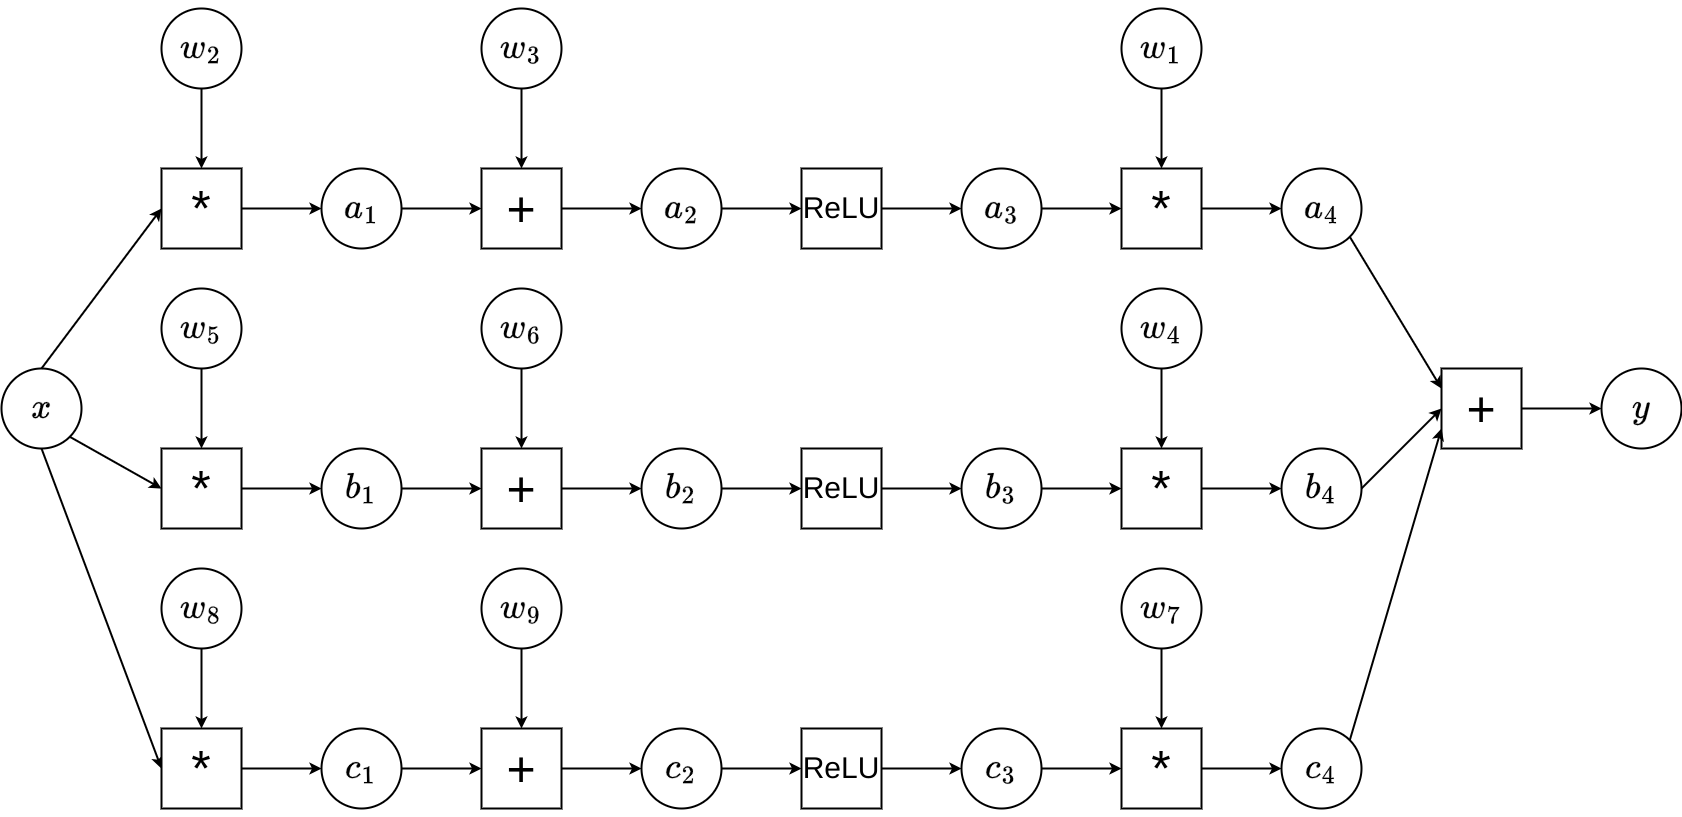
\includegraphics[width=\linewidth]{figures/examnet.png}
        \end{figure}
    \end{solution}
    
    \item For $\theta = (-1, \frac{1}{2}, 0, -4, 1, -2, 4, 1, -5)$, draw the function $y = f(x; \theta)$ for $x \in [-10, 10]$.

    \begin{solution}
        \begin{figure}[h!]
            \centering
            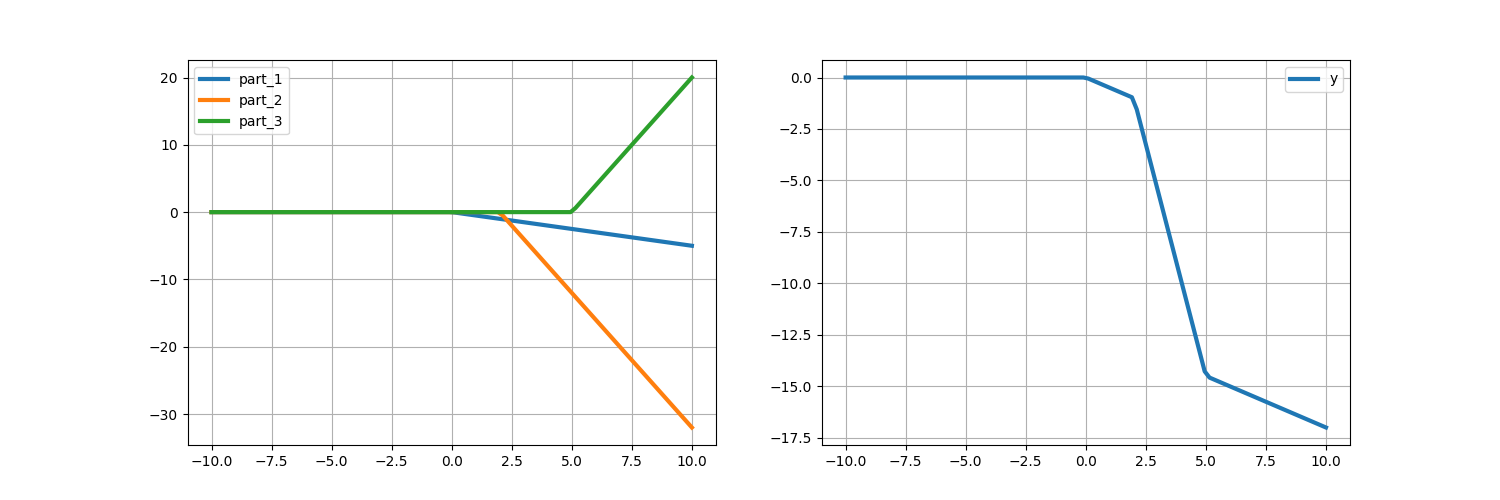
\includegraphics[width=\linewidth]{figures/relunet.png}
        \end{figure}
    \end{solution}
    \newpage
    \item Using the data point $(x, y) = (10, -15)$ and the value of $\theta$ given above, we want to fine-tune the parameter $w_8$ of the neural network such that $f(x; \theta)$ produces a more accurate prediction of $y$.

    \begin{enumerate}
        \item Evaluate the squared error loss at the data point $(x, y) = (10, -15)$ and the current value of $\theta$.
        \begin{solution}
            \begin{align*}
                f(10, \theta) &= -17\\
            \mathcal{L}(\hat{y} &= -17, y=-15) = (17 - 15)^2 = 4    
            \end{align*}
        \end{solution}
        \item Derive an expression for the derivative of the squared error loss with respect to $w_8$.
        \begin{solution}
        The loss is
        $$
        \mathcal{L}(\hat{y}, y) = (\hat{y} - y)^2.
        $$
        We compute the gradient 
        \begin{align*}
            \dfrac{\partial \mathcal{L}}{\partial w_8} &= \dfrac{\partial \mathcal{L}}{\partial \hat{y}}\dfrac{\partial \hat{y}}{\partial c_4}\dfrac{\partial c_4}{\partial c_3}\dfrac{\partial c_3}{\partial c_2}\dfrac{\partial c_2}{\partial c_1}\dfrac{\partial c_1}{\partial w_8}\\
            &= 2(\hat{y} - y)w_7\dfrac{\partial c_3}{\partial c_2}x.
        \end{align*}
        We need to compute forward activations to compute the gradient value. $\dfrac{\partial c_3}{\partial c_2}$ will be 1 if $c_2 > 0$ else $0$ by definition of the ReLU. We have
        \begin{align*}
            \hat{y} &= -17\\
            y &= -15\\
            w_7 &= 4\\
            x &= 10\\
            c_2 &= w_8x + w_9 = 5 \Rightarrow \dfrac{\partial c_3}{\partial c_2} = 1
        \end{align*}
        which gives a gradient equal to $-160$.
        \end{solution}

        \item Update the parameter $w_8$ using one step of gradient descent with a learning rate $\gamma = 0.0005$.
        
        \begin{solution}
            The gradient step is given by
            $$
            w_8 \leftarrow w_8 - \gamma \dfrac{\partial \mathcal{L}}{\partial w_8}
            $$
            which gives an updated $w_8$ equal to $1.08$.
        \end{solution}
        \item Verify that the value of the loss function has decreased after the update.
        
        \begin{solution}
            With the updated $w_8$, we have $\hat{y} = -13.8$ which gives a loss equal to $1.44$. The previous loss value was $4$, we indeed decreased the loss. 
        \end{solution}
    \end{enumerate}
\end{enumerate}

\newpage

\section{Convolution}

Represent the convolution $x \circledast u$ of each of the following signals $x$

\newcommand{\signal}[1]{%
\begin{tikzpicture}
    \begin{axis}[%
        width=8cm,
        height=4cm,
        axis x line=middle,
        axis y line=none,
        domain=0:19,
        samples=20,
        xmin=-1,
        xmax=20,
        ymin=-1,
        ymax=+1,
        xmajorticks=false,
        ymajorticks=false,
    ]
        \addplot+[ycomb,black,thick,mark options={fill=white}] {#1};
    \end{axis}
\end{tikzpicture}
}

\newcommand{\kernel}[1]{%
\begin{tikzpicture}
    \begin{axis}[%
        width=3cm,
        height=4cm,
        axis x line=middle,
        axis y line=none,
        domain=0:3,
        samples=4,
        xmin=-1,
        xmax=4,
        ymin=-1,
        ymax=+1,
        xmajorticks=false,
        ymajorticks=false,
    ]
        \addplot+[ycomb,black,thick,mark options={fill=white}] {#1};
    \end{axis}
\end{tikzpicture}
}

\vspace{1ex}

\signal{2 * (mod(x, 10) < 5) - 1}
\signal{mod(x, 5) / 2 - 1}

\signal{abs(mod(x, 10) - 5) / 2.5 - 1}
\signal{cos(360 * x / 15.29)}

with each of the following convolution kernels $u$.

\vspace{1ex}

\kernel{x / 1.5 - 1}
\kernel{1 - 2 * (x < 2)}
\kernel{1 - 2 * (mod(x, 3) == 0)}

\newpage

\section{Learning to play Pacman (August 2020)}

You observe a Grandmaster agent playing Pacman. How can you use the moves you observe to train your own agent?

\begin{enumerate}
    \item Describe formally the data you would collect, the inference problem you would consider, and how you would solve it.

    \item How would you design a neural network to control your agent? Define mathematically the neural network architecture, its inputs, its outputs, its parameters, as well as the loss you would use to train it.

    \item Discuss the expected performance of the resulting agent when \begin{enumerate*}
        \item the Grandmaster agent is optimal, and
        \item the Grandmaster agent is suboptimal.
    \end{enumerate*}
\end{enumerate}

\newpage

\newpage

\startquiz

We build a MLP with 2 hidden layers of 32 units, ReLU activations and squared error loss. We discard the biases from our linear layers. We know that our input is a vector of 2 elements and the output is a scalar. How much parameters do we have in the network?
\begin{itemize}
    \item 1024.
    \solitem 1120.
    \item 1185.
    \item Another value than the ones proposed above.
\end{itemize}

We add biases in the network proposed above. What is the number of parameters of the network?
\begin{itemize}
    \item Another value than the ones proposed below.
    \item 1089.
    \solitem 1185.
    \item 2048.
    \item 2240.
\end{itemize}

We have an image of shape $(H, W)$, we want to pass it through a layer which reduces each dimension by a constant $K$, i.e. produces an output image of shape $(H-K, W-K)$.
\begin{itemize}
    \item It can be done with a convolution layer with a kernel $(K, K)$ or a linear layer with weight matrix $(HW, (H-K)(W-K))$.
    \solitem It can be done with a convolution layer with a kernel $(K + 1, K + 1)$ or a linear layer with weight matrix $(HW, (H-K)(W-K))$.
    \item It can be done with a convolution layer with a kernel $(K - 1, K - 1)$ or a linear layer with weight matrix $(HW, KK)$.
    \item It can be done with a convolution layer with a kernel $(K+ 1, K+1)$ or a linear layer with weight matrix $(HW, KK)$.
\end{itemize}

From the previous question, we double the number of input pixels by setting the shape of the input image to $(H', W)$ with $H' = 2H$. The latter implies that the output image should be of shape $(H' - K, W - K)$. If only look at weight parameters (no biases)...
\begin{itemize}
    \item The number of parameters of both the linear and convolution layer are doubled. 
    \item The linear layer will have twice more parameters and the convolution twice less.
    \solitem The linear layer will have twice more parameters and the convolution will not change.
    \item Nothing changes neither for the linear layer nor the convolution one.
\end{itemize}

In deep learning, a layer in a multi-layer perceptron is defined as ... 
\begin{itemize}
    \item ${\bf h} = \sigma(\mathbf{W}^T\mathbf{x} + \mathbf{b})$, where $\sigma$ is the standard deviation function.
    \solitem ${\bf h} = \sigma(\mathbf{W}^T\mathbf{x} + \mathbf{b})$, where $\sigma$ is an activation function, such as the sigmoid function.
    \item ${\bf h} = \sigma(\mathbf{W}^T + \mathbf{x} - \mathbf{b})$, where $\mathbf{W} \in \mathbb{R}^{d \times q}$ is matrix of weights.
    \item ${\bf h} = \sigma(\mathbf{W}^T\mathbf{x} + \mathbf{b})$, where $\mathbf{b} \in \mathbb{R}^d$ is the most likely vector of hidden states given $\mathbf{x}$.  
\end{itemize}

Arnaud is trying to perform gradient descent on a function $f(x)$ using the update $$x_{t+1} := x_t - \frac{\partial f}{\partial x}(x_t).$$ Is gradient descent guaranteed to converge to the global minimum of $f$?
\begin{itemize}
    \item Yes, since he's updating using the gradient of $x$.
    \item Yes, but not for the reason above.
    \item No, since he is updating updating $x$ in the wrong direction.
    \solitem No, but not for the reason above. %%% 
\end{itemize}

\end{document}
